\documentclass{beamer}
\usepackage{tikz,amsmath,hyperref,graphicx,stackrel,animate}
\usetikzlibrary{positioning,shadows,arrows,shapes,calc}
\newcommand{\argmax}{\operatornamewithlimits{argmax}}
\newcommand{\argmin}{\operatornamewithlimits{argmin}}
\mode<presentation>{\usetheme{Frankfurt}}
\AtBeginSection[]
{
  \begin{frame}<beamer>
    \frametitle{Outline}
    \tableofcontents[currentsection,currentsubsection]
  \end{frame}
}
\title{Lecture 4: Fourier Synthesis}
\author{Mark Hasegawa-Johnson}
\date{ECE 401: Signal and Image Analysis}
\begin{document}

% Title
\begin{frame}
  \maketitle
\end{frame}

% Title
\begin{frame}
  \tableofcontents
\end{frame}

%%%%%%%%%%%%%%%%%%%%%%%%%%%%%%%%%%%%%%%%%%%%
\section[Spectrum]{Spectrum}
\setcounter{subsection}{1}

\begin{frame}
  \frametitle{Two-sided spectrum}

  The {\bf spectrum} of $x(t)$ is the set of frequencies, and their
  associated phasors,
  \[
  \mbox{Spectrum}\left( x(t) \right) =
  \left\{ (f_{-N},a_{-N}), \ldots, (f_0,a_0), \ldots, (f_N,a_N) \right\}
  \]
  such that
  \[
  x(t) = \sum_{k=-N}^N a_ke^{j2\pi f_kt}
  \]
\end{frame}

%%%%%%%%%%%%%%%%%%%%%%%%%%%%%%%%%%%%%%%%%%%%
\section[Periodic]{Periodic Signals}
\setcounter{subsection}{1}

\begin{frame}
  \frametitle{Fourier's theorem}

  One reason the spectrum is useful is that {\bf\em any} periodic
  signal can be written as a sum of cosines.  Fourier's theorem says that
  any $x(t)$ that is periodic, i.e.,
  \[
  x(t+T_0) = x(t)
  \]
  can be written as
  \[
  x(t) = \sum_{k=-\infty}^\infty X_k e^{j2\pi k F_0 t}
  \]
  which is a special case of the spectrum for periodic signals:
  $f_k=kF_0$, and $a_k=X_k$, and
  \[
  F_0 = \frac{1}{T_0}
  \]
\end{frame}

\begin{frame}
  \frametitle{Analysis and Synthesis}

  \begin{itemize}
  \item {\bf Fourier Analysis} is the process of finding the spectrum,
    $X_k$, given the signal $x(t)$.  I'll tell you how to do that next lecture.
  \item {\bf Fourier Synthesis} is the process of generating the
    signal, $x(t)$, given its spectrum.  I'll spend the rest of
    today's lecture showing examples and properties of synthesis.
  \end{itemize}
\end{frame}

\begin{frame}
  \frametitle{Example \#1: Square wave}

  \centerline{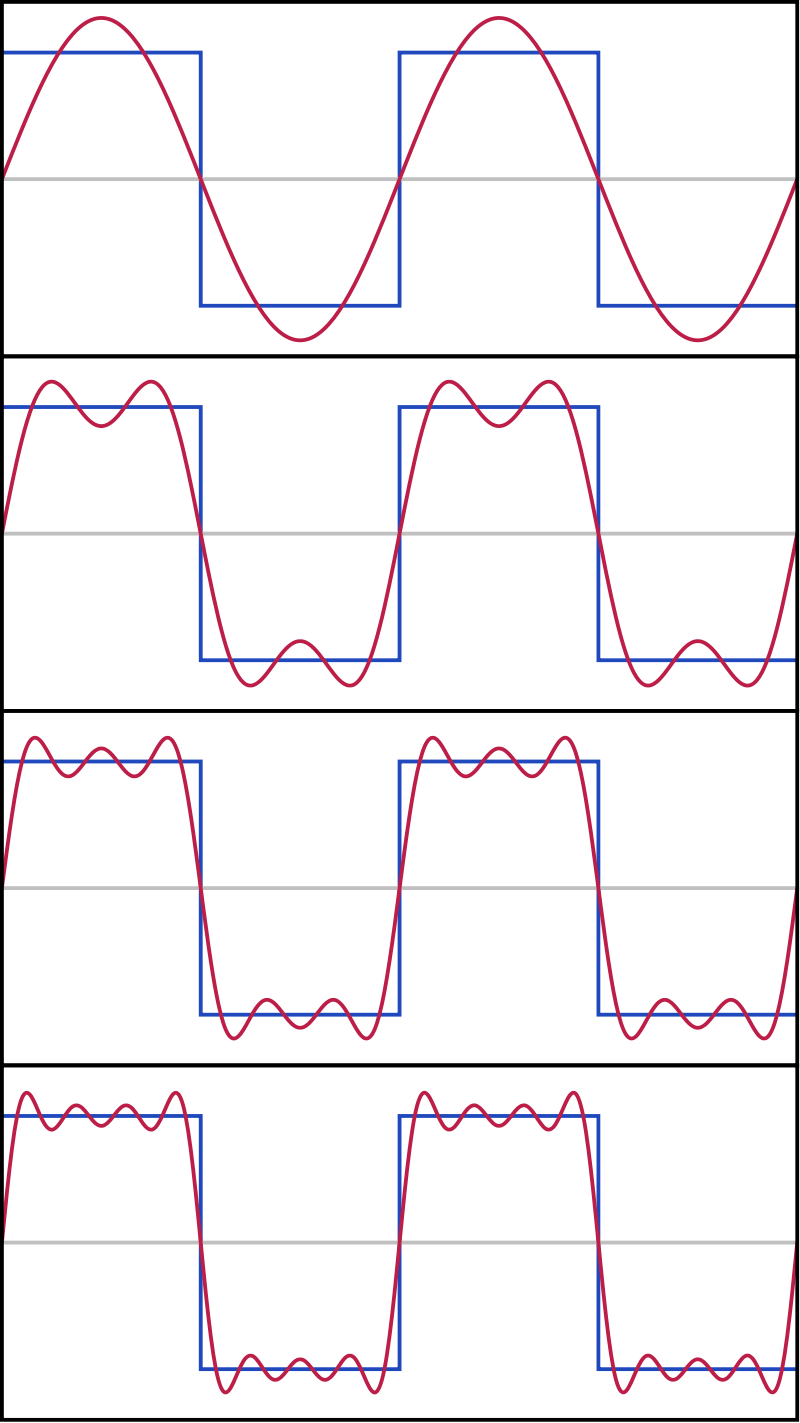
\includegraphics[height=2.5in]{exp/squarewave.png}}
  \begin{tiny}
    Jim.belk, Public domain image 2009,
    \url{https://commons.wikimedia.org/wiki/File:Fourier_Series.svg}
  \end{tiny}
\end{frame}

\begin{frame}
  \frametitle{Example \#1: Square wave\\\begin{tiny}
    \url{https://upload.wikimedia.org/wikipedia/commons/b/bd/Fourier_series_square_wave_circles_animation.svg}\end{tiny}}
    
  \centerline{\animategraphics[loop,controls,height=2.5in]{20}{exp/squarewave_animation-}{0}{59}}
\end{frame}

\begin{frame}
  \frametitle{Example \#2: Sawtooth wave\\\begin{tiny}By Lucas Vieira, public domain 2009,
    \url{https://commons.wikimedia.org/wiki/File:Periodic_identity_function.gif}\end{tiny}}
    
  \centerline{\animategraphics[loop,controls,height=1in]{2}{exp/sawtooth_anim1-}{0}{4}}
\end{frame}

\begin{frame}
  \frametitle{Example \#2: Sawtooth wave\\\begin{tiny}
    \url{https://upload.wikimedia.org/wikipedia/commons/1/1e/Fourier_series_sawtooth_wave_circles_animation.svg}\end{tiny}}
    
  \centerline{\animategraphics[loop,controls,height=2.5in]{20}{exp/sawtooth_anim2-}{0}{59}}
\end{frame}

\begin{frame}
  \frametitle{Example: A weird arbitrary signal\\\begin{tiny}By Scallop7, CC-SA 4.0 2007,
    \url{https://commons.wikimedia.org/wiki/File:Example_of_Fourier_Convergence.gif}\end{tiny}}
    
  \centerline{\animategraphics[loop,controls,height=2.5in]{20}{exp/Fourier_Convergence-}{0}{99}}
\end{frame}

\begin{frame}
  \frametitle{Example: Violin}

  \centerline{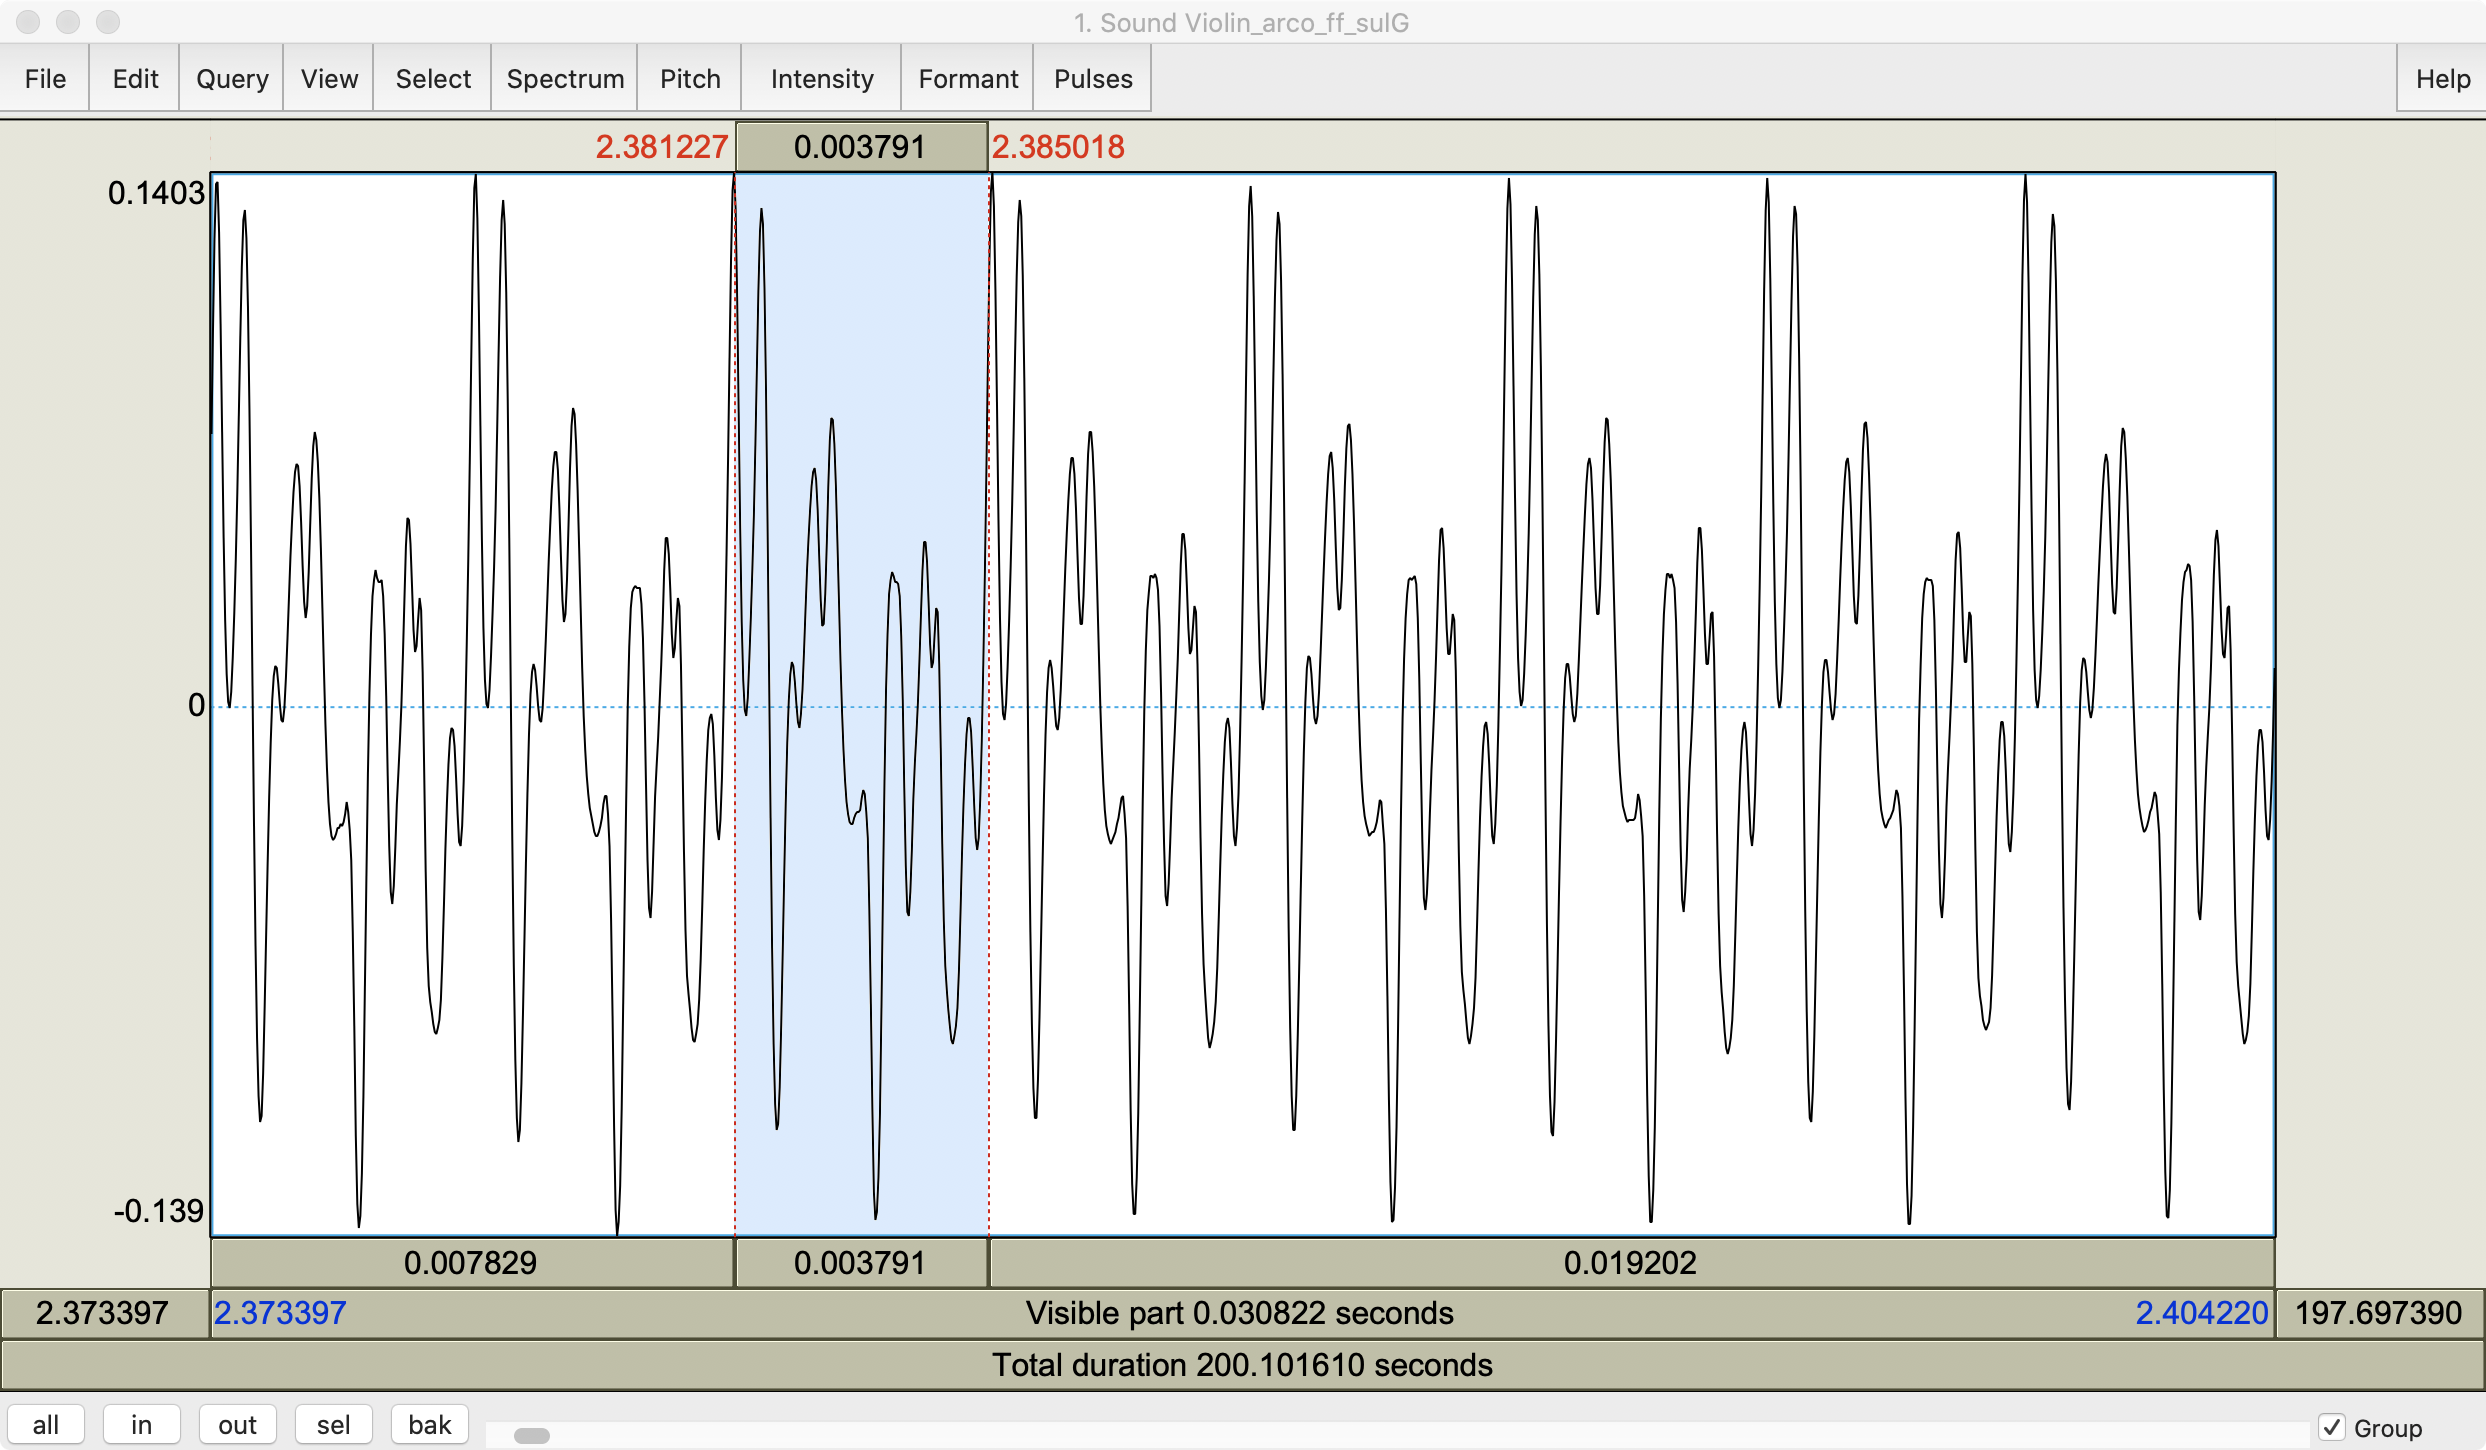
\includegraphics[height=2in]{violin_waveform.png}}
    Eight periods from the recording of a violin playing $f=1/0.003791=262$Hz, i.e., C4 (middle C).
    Waveform distributed by
    \href{http://theremin.music.uiowa.edu/MIS.html}{\bf\color{blue}University of Iowa Electronic Music Studios}.
\end{frame}

\begin{frame}
  \frametitle{Example: Violin}

  \centerline{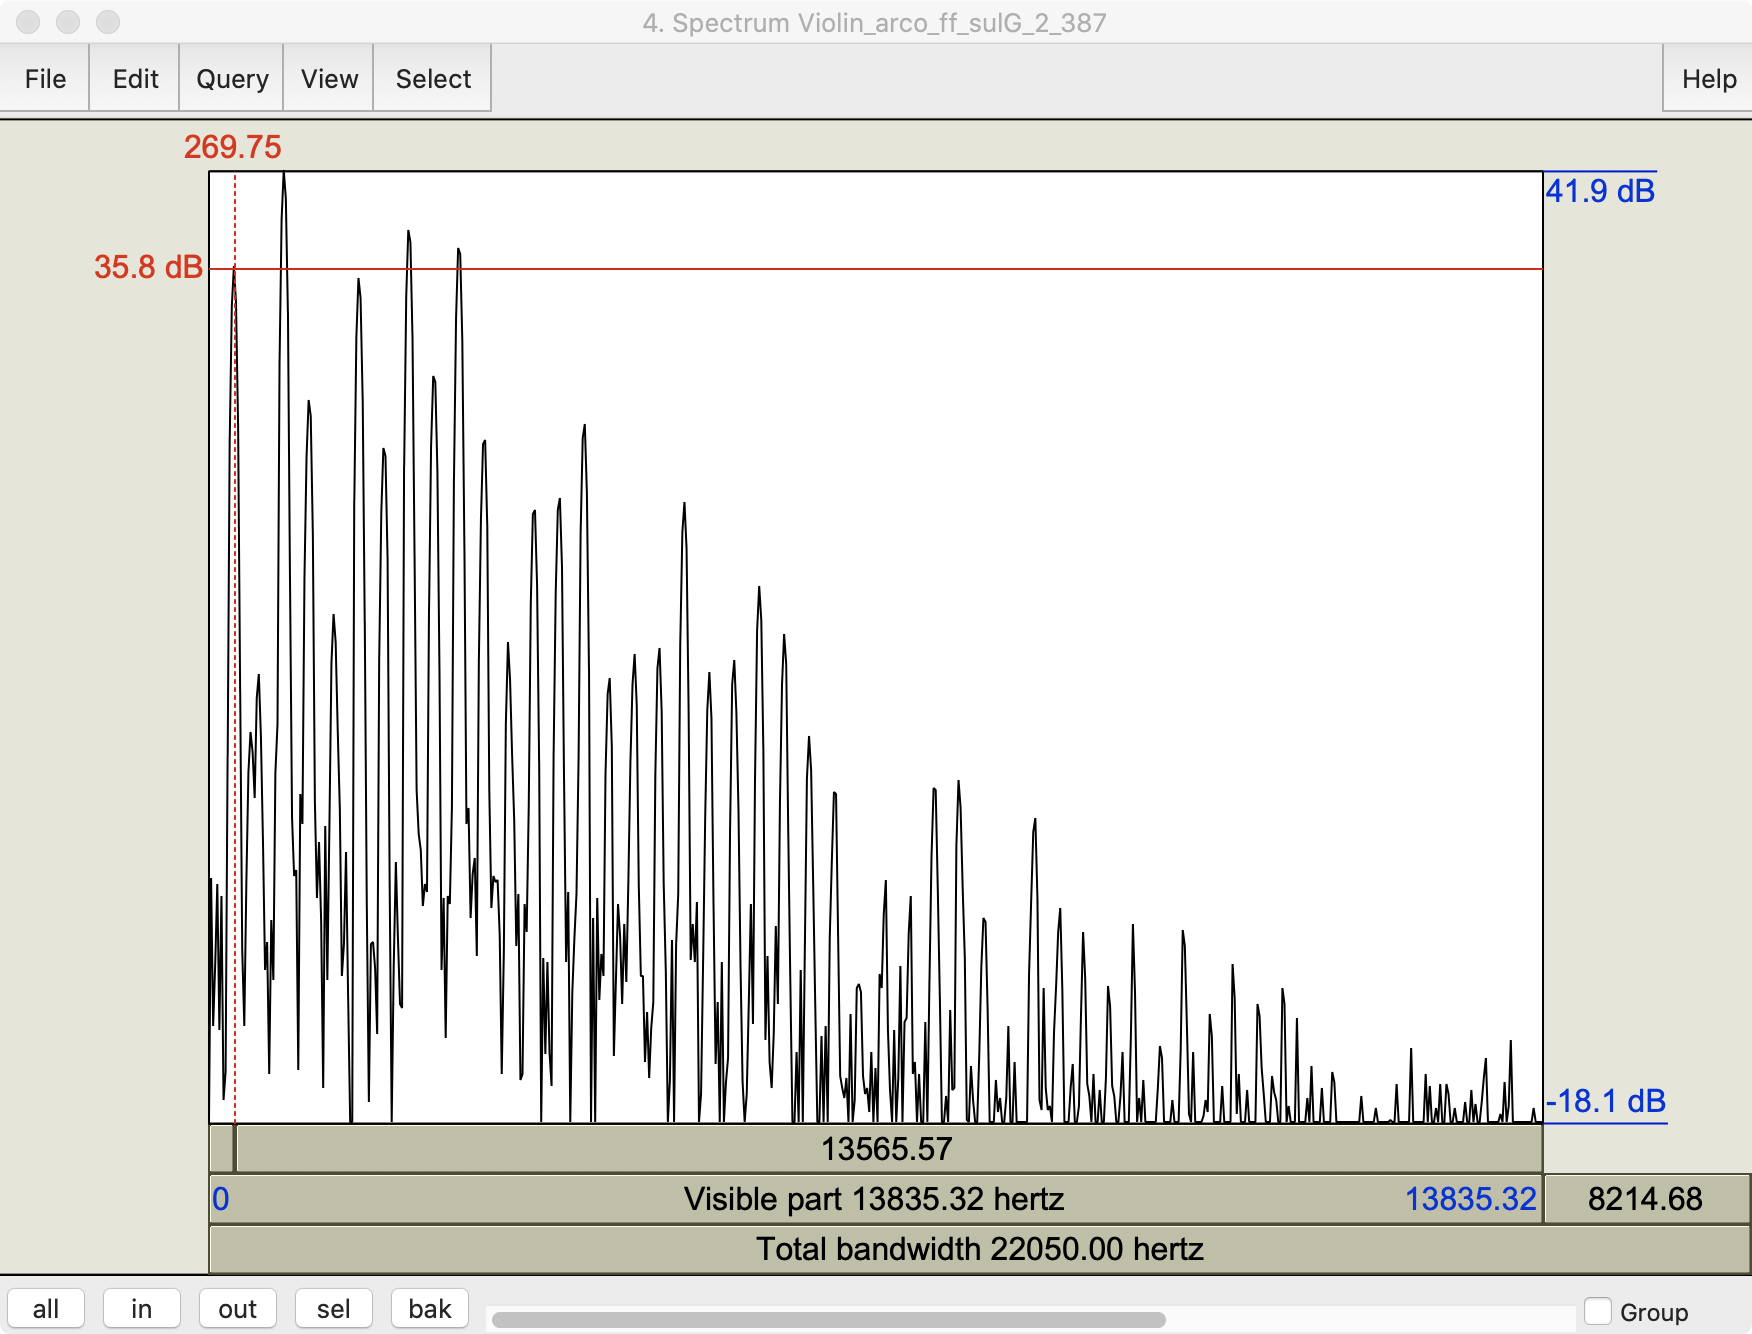
\includegraphics[height=2.5in]{violin_spectrum.png}}
    Log magnitude spectrum ($20\log_{10}|X_k|$) for the first 43 harmonics or so
    ($1\le k\le 43$ or so) of a violin playing C4.
    Waveform distributed by
    \href{http://theremin.music.uiowa.edu/MIS.html}{\bf\color{blue}University of Iowa Electronic Music Studios}.
\end{frame}

%%%%%%%%%%%%%%%%%%%%%%%%%%%%%%%%%%%%%%%%%%%%
\section[Pitch]{Pitch}
\setcounter{subsection}{1}

\begin{frame}
  \frametitle{The missing fundamental}

  Suppose we have a signal of the form
  \[
  x(t) = \sum_{k=-\infty}^{\infty} X_k e^{j2\pi k F_0 t}
  \]
  Humans will hear the frequency $F_0$ to be the pitch of this sound,
  even if $X_{-1}=X_1=0$, i.e., even if the sound has no energy at the
  frequency $F_0$.
  
\end{frame}

\begin{frame}
  \frametitle{The missing fundamental}

  Our visual perception matches auditory perception. For example:
  \centerline{\includegraphics[height=2in]{exp/missing_fundamental.jpg}}
  {\small CC-SA 3.0, \url{https://commons.wikimedia.org/wiki/File:Illustration_of_common_periodicity_of_full_spectrum_and_missing_fundamental_waveforms.jpg}}
  
\end{frame}

\begin{frame}
  \frametitle{Quiz}

  Try the quiz! Go to the course webpage, and click on today's date.
\end{frame}

\begin{frame}
  \frametitle{The autocorrelation theory of pitch perception}

  The mystery of the missing fundamental was solved by Licklider in
  1951.  He showed that we can explain why humans hear $F_0$ as the
  pitch if we assume that humans use the following strategy:
  \begin{enumerate}
  \item Your ear divides the sound into separate harmonics, each of
    which is tracked by a perceptual neuron.
  \item The $k^{\text{th}}$ perceptual neuron synapses onto a timer
    neuron in some way that removes the phase of the harmonic, i.e.,
    it creates a signal $y(t)$ whose harmonic amplitudes are
    $Y_k=|X_k|$, the absolute value.
  \item Finally, a third neuron adds together all of the zero-phase
    harmonics.
  \end{enumerate}
\end{frame}

\begin{frame}
  \frametitle{The autocorrelation theory of pitch perception}

  Suppose $Y_k$ are all positive real numbers (zero phase).  Then
  \begin{align*}
    \sum_{k=-K}^K Y_k e^{j2\pi kF_0t}
    &=  Y_0+ \sum_{k=1}^K 2Y_k\cos\left(2\pi kF_0t\right)\\
    &\stackbin[K\rightarrow\infty]{}{\rightarrow}
    \left\{\begin{array}{ll}
    \infty & t=0,T_0,2T_0,\ldots\\
    0 &\mbox{otherwise}
    \end{array}\right.
  \end{align*}
  \centerline{\includegraphics[height=1in]{exp/impulsetrain.png}}
\end{frame}

\begin{frame}
  \frametitle{The autocorrelation theory of pitch perception}

  \centerline{\includegraphics[height=2in]{exp/rectangles.png}}
  {\small CC-SA 3.0, \url{https://commons.wikimedia.org/wiki/File:Missing_fundamental_rectangles.svg}}
\end{frame}

%%%%%%%%%%%%%%%%%%%%%%%%%%%%%%%%%%%%%%%%%%%%
\section[Summary]{Summary}
\setcounter{subsection}{1}

\begin{frame}
  \frametitle{Summary}
  \begin{itemize}
  \item {\bf Fourier's Theorem:} Any periodic waveform,
    $x(t+T_0)=x(t)$, can be synthesized as
    \[
    x(t) = \sum_{k=-\infty}^\infty X_ke^{j2\pi kF_0t}
    \]
  \item {\bf Autocorrelation theory of pitch perception:} If all of
    the $Y_k$ are positive real numbers, then
    \begin{align*}
      \sum_{k=-K}^K Y_k e^{j2\pi kF_0t}
      &=  Y_0+ \sum_{k=1}^K 2Y_k\cos\left(2\pi kF_0t\right)\\
      &\stackbin[K\rightarrow\infty]{}{\rightarrow}
      \left\{\begin{array}{ll}
      \infty & t=0,T_0,2T_0,\ldots\\
      0 &\mbox{otherwise}
      \end{array}\right.
    \end{align*}
  \end{itemize}
  
\end{frame}

\end{document}
